\documentclass[lang=en,color=green]{elegantbook}
\title{Pragmatic Node.js development}
\subtitle{Primer in Nest.js}

\author{Zlatibor Zed Veljkovic}
\date{June 5, 2022}
\version{0.1}
\bioinfo{bioinfo 1}{bioinfo 2} 

\extrainfo{Some extra info}

\setcounter{tocdepth}{3}


\logo{cule.jpg}
\cover{cover.jpg}
 
\definecolor{codebg}{rgb}{0.8,0.8,0.8}
        
% 本文档命令
\usepackage{array}
\usepackage{enumitem}
\usepackage{minted}
\usepackage{mdframed}
\newcommand{\ccr}[1]{\makecell{{\color{#1}\rule{1cm}{1cm}}}}
\newcommand{\ci}{\mintinline{bat}}
\newcommand{\bi}[1]{\textit{\textbf{#1}}}
\setmintedinline{bgcolor=codebg}
% 修改标题页的橙色带 
% \definecolor{customcolor}{RGB}{32,178,170}
% \colorlet{coverlinecolor}{customcolor}

\begin{document}

\maketitle
\frontmatter

\tableofcontents

\mainmatter

\chapter{Developer tools}

Since ancient times, mankind has constantly spent effort to create new or to improve existing tools. 
Even now, after thousands and thousands of years we are doing the same. 
We are making new tools that will make us more efficient or at least to do our tasks easier.
In software development there are so many tools available it is hard to choose which set should be used. Next sections will give simple overview of most prominent tools for each section. 


\section{Command line interfaces}
Commad line interfaces (CLI) are programs that use textual interface and allow you to interact with it. 
Every operating system comes with one or more of these, Windows has Command Prompt (aka cmd.exe) and Power Shell,
Linux has sh and bash with many alternatives (commonly known as shell), and Mac OS has Terminal.app. 
One issue that novice developers struggle is that when someone tells you to “open the terminal”,
they mean one for your system. 

Before mentioned apps are the ones that allow you to execute some commands or run different programs.
There are also some CLI that is specifically built for one purpose. 
One example would be Nest.js CLI which allows you to quickly create new projects,
 update dependencies or start the Nest app. 

\subsection{Command prompt} 
Command prompt comes preinstalled on Windows systems.
It supports batch scripts and usually the file is with .bat extension.

\noindent\begin{minipage}[t]{0.5\textwidth}%
    \centering{Pros} 
    \begin{itemize}[leftmargin=*]
        \item Available on all Windows systems
        \item Allows executing programs in current directory without  \lstinline{.\}  prefix
    \end{itemize}
\end{minipage}%
\begin{minipage}[t]{0.5\textwidth}%
    \centering{Cons} 
    \begin{itemize}[leftmargin=*]
        \item Batch scripting language is really outdated and hard to write more complex stuff
        \item No command history search
    \end{itemize}
\end{minipage}%

\begin{figure}[htbp]
    \centering
    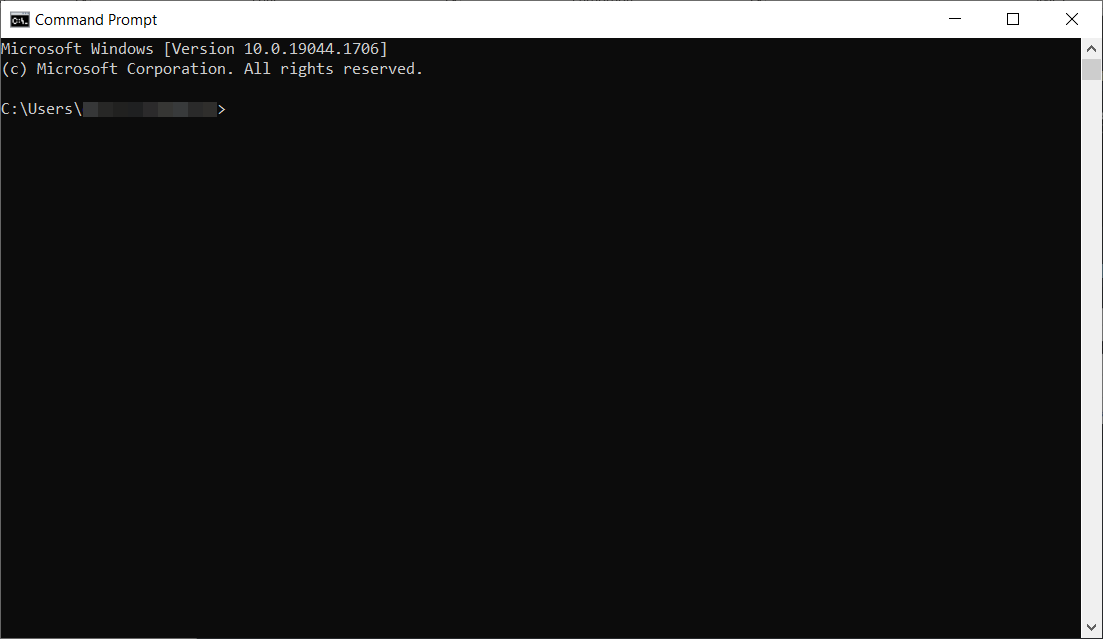
\includegraphics[width=0.6\textwidth]{images/command-prompt.png}
    \caption{Command Prompt\label{fig:Command Prompt}}
\end{figure}

Reference for available Command Prompt commands can be found at \href{https://docs.microsoft.com/en-us/windows-server/administration/windows-commands/windows-commands}{Windows Commands}

\subsection{PowerShell} 
Another shell for Windows systems is called PowerShell and it is available from
Windows 7 or later operating systems. Open source version PowerShell Core was released in 2016 and  
it is based on .Net Core which also made it cross-platform. It has better integration
with various functionalities available in Windows so it is prefreed choice over Command Prompt
when working with system administration. For developer work it might be an overkill.


\noindent\begin{minipage}[t]{0.5\textwidth}%
    \centering{Pros} 
    \begin{itemize}[leftmargin=*]
        \item Available on all Windows systems
        \item Better integration with Windows functionalities
        \item Has command history search (with F8 key)
    \end{itemize}
\end{minipage}%
\begin{minipage}[t]{0.5\textwidth}%
    \centering{Cons} 
    \begin{itemize}[leftmargin=*]
        \item  Does not allow executing programs in 
        current directory without  \lstinline{.\} prefix
    \end{itemize}
\end{minipage}%

\begin{figure}[htbp]
    \centering
    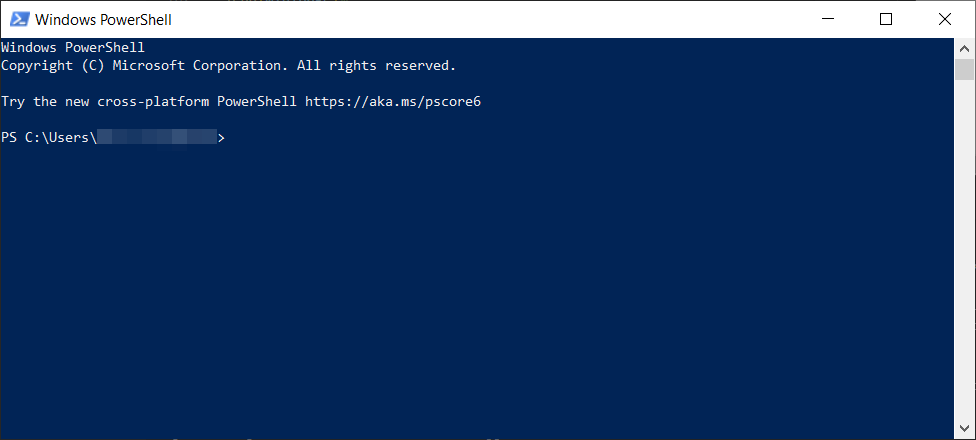
\includegraphics[width=0.6\textwidth]{images/powershell.png}
    \caption{PowerShell\label{fig:PowerShell}}
\end{figure}

\subsection{Linux/Mac terminals/shells}

Linux and Mac have much bigger choice of terminals. Terminal refers to a program that allows you to run
programs which are known as shells. Shells come in lots of varieties sh, bash, ksh, csh, zsh\dots. 
Linux has many command line programs that allow you to manipulate output of commands and 
offers a lot for power users.


\section{Package managers} 

Package managers can be used to install additional software on your PC. They usully automate process of 
downloading, installing and configuring software. Later it also helps with keeping the installed software 
up to date or with removal. 

\begin{itemize}[leftmargin=*]
    \item Chocolatey is most prominent Windows package manager. It can be downloaded from \href{https://chocolatey.org/}{https://chocolatey.org/}.
    Searching for packages is done with \mintinline{bat}{choco search postgresql} 
    and installation with \mintinline{bat}{choco install postgresql} will install Postgres.
    \item Homebrew is a Mac OS X package manager written in Ruby. 
    It can be downloaded from \href{https://brew.sh}{https://brew.sh}.
    Command \mintinline{bat}{brew search postgres}
    is used to search for package while \mintinline{bat}{brew install postgresql} to install a package.
    \item Linux has many package managers and preferred way is to use package manager
    that comes with operating system.
\end{itemize}

\chapter{NestJS application recommendations}

\section{NestJS}

I couldnt explain it better then the words of the author "Nest (NestJS) is a framework for building 
efficient, scalable Node.js server-side applications.
It uses progressive JavaScript, is built with and fully supports
TypeScript (yet still enables developers to code in pure JavaScript)
and combines elements of OOP (Object Oriented Programming), 
FP (Functional Programming), and FRP (Functional Reactive Programming)."

The documentation is found on \href{https://docs.nestjs.com/} where you can 
read all about framework components. Some of the components are  
not up to task and in further sections we will focus on good and bad 
sides of available components and some alternatives.

\section{Environments}
Modern apps usually run in multiple environments. My recommendation 
for environments is with code name in parenthesis.

\begin{itemize}
    \item Local development environment (\bi{a})
    \item Local testing environment (\bi{b})
    \item Public development environment (\bi{d})
    \item Public stable development environment (\bi{s})
    \item CI testing environment (\bi{t})
    \item Public quality assurance environment (\bi{q})
    \item Public production environment (\bi{p})
\end{itemize}

\subsection{Local development environment}
Local development environment is pretty obvious as each developer 
is running the application on development machine.
Code name to be used for this environment is \bi{a} which as a letter
represents first letter in alphabet so this environment represents 
first step in the application development.

\subsection{Local testing environment}
Local testing environment (\bi{b}) is where developer runs tests on development
machine. This environment is necessery to isolate testing of the app
completly from local development environment. Without this isolation
data that has been entered during development could influence
test running. We usually use same variables
as \bi{a} env but we usually want to change external dependencies
like database/queues/Kafka/storage so test runs are properly isolated.

\subsection{Public development environment}
Public development environment is the environment which contains the
latest application code. It is configured to be automatically built 
from the \bi{develop} branch. This environment is meant to be 
broken/reset at any time. It is also first public environment for use 
mostly by developers.

\subsection{Public stable development environment}
Public stable development environment \bi{s} is the environment that is 
manually updated. When team is happy with the state of \bi{d} environment
they can promote it to this environment. This allows team leads 
to test the app without interuptions that would come if they used \bi{d} 
environment.

\subsection{CI testing environment}
CI testing environment is used during the PR verifications in the build
pipelines. This is necessary for same reasons as local testing environment,
just on the public side. 

\subsection{Public quality assurance environment}
Public quality assurance environment \bi{q} is environment meant
for external evaluation. When all issues identified in \bi{s} environment
are fixed and team lead is happy with it's state, this build can be promoted
to \bi{q} environment. This environment should be same in specs as 
public production environment, so it can be also used as database
migration verification or as performnce test target. 

\subsection{Public production environment}
Public production environment \bi{p} is environment that is available to the 
users of the application. This makes it last step in build - release cycle.
As real users are using it this environment should be under constant monitoring.

\section{Environment zones}
All of the enivornments can be grouped in production and non-production zones.
The app code can then provide developers with:
\begin{itemize}
    \item More information about errors for example by outputing
 stack traces, displaying error data, and various other info which should be
 hidden from the real users.
    \item Improve testability by including features to login as certain type
    of users, commands that will precreate certain data sets, etc\dots
    \item Distinguish between seeding production data and developer data.
\end{itemize} 


\section{Application Configuration}

Application configuration in modern development is unescapable. NestJS 
offers a component \bi{ConfigService} which is using \bi{dotenv} package internally.
What we get is a way to load .env environment file and access the variables
defined in environment.

What we are missing is:
\begin{itemize}
    \item Checking that all required variables are supplied
    \item That variables conform to the expected type (configuration schema)
    \item Ability to use multiple .env files so that you can easily configure 
    local development environment (\bi{a}) and local testing environment (\bi{b})
    for example by having \bi{.env.b} file overriding database name from \bi{.env} 
    used by local development environment.
    \item Type safety as we need to use string identifiers when getting the 
    values
\end{itemize}

Package \href{https://www.npmjs.com/package/convict}{convict} has almost all
of the above but has a requirement that each setting has default value 
which will not fail the startup if required variable is not found in 
environment variables.

\section*{Zeddy Config}
Zeddy Config is my \href{https://www.npmjs.com/package/zeddy-config}{library} 
heavily inspired by \href{https://www.npmjs.com/package/convict}{convict} but offers 
type safety without default values and is offering just enough functionality
for any app. This package also provides variable loading from the \bi{.env} 
and \bi{.env.env-name} files with the \bi{dotenvize} method. With this simple
packages we cover all missing elements for good conifg:
\begin{itemize}
    \item Single method load the environment variables into JS variable.
    \item Validation of the configuration schema.
    \item Full type safety as schema type propery is trasferred to config object properties.
    \item It also has additional method to load multiple .env files (\bi{dotenvize}).
\end{itemize}

\begin{minted}{javascript}
import { configz, dotenvize } from "zeddy-config";

dotenvize();

export const config = configz({
  env: {
    description: "Running environment",
    envVar: "NODE_ENV",
    type: "string"
  },
  server: {
    description: "Server info",
    type: "object",
    properties: {
      port: {
        description: "Server port",
        envVar: "SERVER_PORT",
        type: "int",
        validator: (port) => {
          return port === 3000;
        }
      },
      host: {
        description: "Server host",
        envVar: "SERVER_HOST",
        type: "string"
      },
    }
  }
});

// resulting config interface is {env: string; server: {port: number; host: string}}
}
\end{minted}



\end{document}